\documentclass[10pt,twocolumn,letterpaper]{article}
\usepackage[review]{cvpr}
%% This file contains a number of tweaks that are typically applied to the main document.
%% They are not enabled by default, but can be enabled by uncommenting the relevant lines.


%%
%% Official support for 2-column teaser figure
%%
\usepackage{cuted} %< for strip environment

%%
%% For auto-referencing of figures (see fig/teaser.tex and \label{} therein) 
%%
\usepackage{currfile} %< for \currfilebase macro

%%
%% caption and (global) spacing overrides
%%
\usepackage{caption} %< for "\captionof" commands (teaser)
% \setlength{\abovecaptionskip}{.5em} % space above caption
% \setlength{\belowcaptionskip}{1em} % space below caption

%%
%% Inline annotations; for predefined colors, refer to "dvipsnames" in the xcolor package:
%% https://tinyurl.com/overleaf-colors
%%
\newcommand{\red}[1]{{\color{red}#1}}
\newcommand{\todo}[1]{{\color{red}#1}}
\newcommand{\TODO}[1]{\textbf{\color{red}[TODO: #1]}}
%%
%% Disable for camera ready / submission by uncommenting these lines:
%%
% \renewcommand{\TODO}[1]{}
% \renewcommand{\todo}[1]{#1}

%%
%% Work harder in optimizing text layout. Typically shrinks text by 1/6 of page, enable
%% it at the very end of the writing process, when you are just above the page limit.
%%
% \usepackage{microtype}

%%
%% Fine-tune paragraph spacing.
%%
% \renewcommand{\paragraph}[1]{\vspace{.5em}\noindent\textbf{#1.}}

%%
%% Globally adjusts space between figure and caption.
%%
% \setlength{\abovecaptionskip}{.5em}

%%
%% Allows "the use of \paper to refer to the project name"
%% with automatic management of space at the end of the word.
%%
% \usepackage{xspace}
% \newcommand{\paper}{ProjectName\xspace}

%%
%% Commonly used math definitions.
%%
% \DeclareMathOperator*{\argmin}{arg\,min}
% \DeclareMathOperator*{\argmax}{arg\,max}

%%
%% Tighten underline.
%%
% \usepackage{soul}
% \setuldepth{foobar}

%%
%% Reconfigure paragraph (tweaks spacing)
%%

\definecolor{cvprblue}{rgb}{0.21,0.49,0.74}
\usepackage[breaklinks,colorlinks,allcolors=cvprblue]{hyperref}
\usepackage{graphicx,amsmath,amssymb,booktabs}
\def\confName{CVPR}
\def\confYear{2027}
\title{Converting Graph Neural Networks for Graph-Structured Vision: Exact Error Identity, Membrane Readout, and an Accuracy--Energy Frontier on Superpixel Graphs}
\author{Anonymous Submission --- Paper ID *****}
% AUTO-GENERATED by protocols/gen_paper_artifacts.py from results/*.json.
% Do not edit by hand.
\newcommand{\MACPJ}{4.6}
\newcommand{\ACPJ}{0.9}
\newcommand{\MACACRatio}{5.11}
\newcommand{\TotalSeeds}{20}
\newcommand{\IdentityMax}{1.21e-14}
\newcommand{\IdentityMin}{4.88e-15}
\newcommand{\FloatGap}{3.7\times10^{-7}}
\newcommand{\MNISTAnn}{34.02}
\newcommand{\MNISTLoss}{3.79}
\newcommand{\MNISTLossStd}{2.26}
\newcommand{\MNISTEp}{9.103}
\newcommand{\MNISTEc}{6.086}
\newcommand{\CIFARAnn}{27.27}
\newcommand{\CIFARLoss}{1.57}
\newcommand{\CIFARLossStd}{0.67}
\newcommand{\CIFAREp}{7.603}
\newcommand{\CIFAREc}{5.938}
\newcommand{\CIFARLower}{0.983}
\newcommand{\EIGHTEENMNISTLoss}{7.29}
\newcommand{\EIGHTEENCIFARLoss}{2.27}
\newcommand{\BetaLossVoneM}{14.64}
\newcommand{\BetaLossVtwoM}{3.10}
\newcommand{\BetaLossVoneC}{13.31}
\newcommand{\BetaLossVtwoC}{2.13}
\newcommand{\MarginMNIST}{43.67}
\newcommand{\MarginCIFAR}{19.85}
\newcommand{\EarlierConsA}{5.405}
\newcommand{\EarlierConsB}{5.725}
\newcommand{\FourthCons}{5.870}
\newcommand{\MinCons}{5.464}
\newcommand{\MembraneAcc}{65.79}
\newcommand{\CountAcc}{16.54}
\newcommand{\TPPGain}{19.82}

% The author-kit review ruler is drawn by lineno into the gutter in
% two-column mode and overlaps body text. Keep the review/confidential
% header but suppress the intrusive line numbers for readability.
\AtBeginDocument{\nolinenumbers}
\newcommand{\Bh}{\hat{B}}
\newcommand{\RAEW}{R A(E_1W_2)}
\begin{document}
\maketitle
\begin{abstract}
ANN-to-SNN conversion is analysed almost exclusively on row-stochastic convolutional operators. We transfer a conversion framework originally assembled for graph node classification to graph-structured visual classification, where images ship as superpixel graphs. A fixed linear global pooling operator preserves the exact conversion-error identity $\hat{B}-B=R A(E_1W_2)$, which we verify to machine precision with a unified float64 forward pass. We find that the closed-form bias $\beta^\star=\theta/(2T)$ becomes redundant once spike trains are deterministic and that removing it substantially improves fidelity. With membrane decoding, margin regularisation and narrow low-timestep networks, both 45\,nm arithmetic-energy conventions exceed $5\times$ across four mutually disjoint holdout groups (20 independent seeds), while all adapted single-point conversion baselines remain near chance. We report the accompanying accuracy--energy frontier explicitly, including a negative scaling result, rather than claiming a simultaneous fidelity target. Energy figures are theoretical op-count estimates, not hardware measurements.
\end{abstract}
\section{Introduction}
\label{sec:intro}

Graph neural networks (GNNs) are increasingly used as vision backbones: an image is represented as a set of superpixels or patches connected by a spatial adjacency, and message passing replaces the regular convolutional grid~\cite{dwivedi2023,han2022vig,achanta2012}. This representation is attractive for irregular objects and for event-driven deployment, yet the ANN-to-SNN conversion theory that makes spiking inference cheap was developed almost entirely for row-stochastic convolutional operators~\cite{diehl2015,rueckauer2017,sengupta2019,deng2021,bu2022qcfs}. For a graph, the propagation operator is neither a grid nor necessarily row-stochastic, and its row sums depend on degree and edge weight. Whether a conversion recipe calibrated for convolutions remains valid on such operators is largely untested.

A second, more practical gap concerns energy. Spiking inference replaces multiply--accumulates (MACs) with accumulations (ACs); under a 45\,nm model the per-operation ratio is only \MACACRatio~\cite{horowitz2014}. Consequently a $5\times$ arithmetic-energy advantage requires the total number of synaptic operations to fall below the ANN's MAC count, not merely to replace some of them. Most conversion studies report accuracy--latency curves on CNNs or ImageNet-scale models~\cite{wu2024ftbc,bojkovic2025tpp,hao2025parallel,huang2025dcgs}, and spike counts on graphs are rarely converted into an explicit ANN-relative energy statement with two independent accounting conventions.

This paper studies a combination of conversion components that was originally assembled for graph node classification, and asks whether that combination transfers to \emph{graph-structured visual classification}. Our starting point is a two-layer GCN with an exact conversion-error identity $\Bh - B = \RAEW$, a closed-form forward bias $\beta^\star=\theta/(2T)$, a membrane-potential readout, and a margin-recovery bound. We do \emph{not} claim to invent these individual components: threshold balancing, zero-expected-error bias, membrane decoding, deterministic counting and two-phase neurons all have their own lineage~\cite{deng2021,bu2022qcfs,wu2024ftbc,dualphase2024,bojkovic2025tpp,ramesh2025pascal}. Our contribution is the \emph{re-identification and adaptation of the combination} on a new operator class: we show that a linear global pooling matrix preserves the identity exactly, that the closed-form bias becomes redundant and harmful once the spike train is deterministic, and that margin regularisation plus a narrow, low-timestep network reaches a stable arithmetic-energy advantage while keeping the conversion fidelity measurable.

Specifically, we make four contributions.

\begin{itemize}
\item \textbf{Exact identity with a graph-level readout.} For a block-diagonal superpixel adjacency $A$ and a linear pooling matrix $R$, the conversion error is exactly $\Bh-B = R A (E_1 W_2)$ with $E_1 = c_1/T - \operatorname{ReLU}(B_1)$. We verify this identity to \IdentityMax\ with a unified float64 forward pass, and show that the residual observed under float32 is an accumulation artefact rather than a theoretical failure.
\item \textbf{A mechanism-level correction of the combination.} Deterministic two-phase spiking already realises the target firing count exactly ($\sum_t s[t]=n$). Adding $\beta^\star=\theta/(2T)$, which compensates floor-quantisation bias, double-corrects the rate. Removing it reduces the $T{=}8$ conversion loss from \BetaLossVoneM\ to \BetaLossVtwoM\ on MNIST superpixels and from \BetaLossVoneC\ to \BetaLossVtwoC\ on CIFAR10 superpixels, across five seeds.
\item \textbf{A stable arithmetic-energy result.} Across four mutually disjoint holdout groups (\TotalSeeds\ independent seeds), the converted network exceeds $5\times$ under both energy conventions on both datasets, without a single seed-level exception. Section~\ref{sec:experiments} reports the ratios and the margins over every adapted single-point baseline.
\item \textbf{An explicit accuracy--energy frontier.} Rather than optimising a single operating point, we characterise how conversion loss trades against energy and include a negative result: a larger training budget worsens fidelity at low timestep counts. The frontier, not a post-hoc operating point, is the object of study.
\end{itemize}

Energy numbers are 45\,nm \emph{theoretical arithmetic op-count estimates}, not measured joules on neuromorphic hardware. Because the energy constraint forces a narrow network, teacher accuracies (\MNISTAnn\% and \CIFARAnn\%) are modest; the evaluation therefore concerns conversion fidelity and energy rather than classifier quality. The method covers fixed, non-negative, linear adjacency with linear pooling; dynamic attention, nonlinear pooling and ImageNet-scale training fall outside its scope.

\section{Related Work}
\label{sec:related}

\textbf{ANN-to-SNN conversion.} Rate-based conversion replaces rectifiers with integrate-and-fire units and interprets firing rates as activations. Weight/threshold balancing, data-based normalisation, reset-by-subtraction and soft reset established the basic pipeline~\cite{diehl2015,rueckauer2017,sengupta2019,han2020rmp}. Deng and Gu derived a layerwise recursion and the closed-form bias that removes the systematic rate offset~\cite{deng2021}; QCFS replaced ReLU with a quantised clip--floor--shift activation so that the expected conversion error vanishes~\cite{bu2022qcfs}. FTBC added a forward temporal bias~\cite{wu2024ftbc}, and an optimal-transport view of the same correction was developed in~\cite{bojkovic2024ot}. Dual-Phase decoding showed that reading the membrane potential avoids the $1/T$ quantisation grid~\cite{dualphase2024}. TPP introduced two-phase probabilistic neurons to exploit temporal misalignment~\cite{bojkovic2025tpp}; PASCAL used inhibitory spikes for deterministic exact counting~\cite{ramesh2025pascal}; parallel spiking conversion, differential coding, adaptive bursts, channel-wise softplus thresholds, error-compensation learning and adaptive fission target the low-latency regime~\cite{hao2025parallel,huang2025dcgs,wang2025adafire,yang2025csqcfs,liu2025ecl,jiang2025fission}. Recent preprints continue to refine residual-membrane alignment, group-wise thresholds and fine-tuning~\cite{chen2026rmp,ji2026gtdl,xia2026neuro}. All of these are developed and evaluated on convolutional or attentional vision backbones with row-stochastic operators.

\textbf{Spiking graph networks.} Spiking GCNs are overwhelmingly trained directly with surrogate gradients~\cite{neftci2019,fang2023spikingjelly}, and large-scale evaluations of spiking GNNs contain no conversion method~\cite{sgnnbench2025}. One-Spike SNN converts both CNNs and text GCNs with single-spike phase coding~\cite{hwang2025onespike}, but does not analyse conversion error for message passing or compare ANN-relative energy. To our knowledge, no published work transfers a full conversion-error formulation to graph-level visual classification and evaluates it against a complete family of conversion baselines.

\textbf{Graph-structured vision.} Vision GNNs build $k$-NN graphs over image patches~\cite{han2022vig,knyazev2019}, while superpixel graph benchmarks convert MNIST and CIFAR10 images into 40--150-node graphs using SLIC and an 8-NN Gaussian-weighted adjacency~\cite{dwivedi2023,achanta2012}. These datasets ship \emph{with} their graph structure, which makes them a direct test bed: no graph construction or freezing heuristic is needed, and the propagation operator is fixed and non-negative. Classical graph backbones and semi-supervised splits provide the architectural substrate~\cite{kipf2017,velickovic2018,hamilton2017,yang2016planetoid}.

\textbf{Energy accounting.} SNN energy studies typically count synaptic operations and apply a 45\,nm CMOS table in which a 32-bit MAC costs \MACPJ\,pJ and an AC costs \ACPJ\,pJ~\cite{horowitz2014,eshraghian2023}. Because this ratio is only \MACACRatio, an advantage of $5\times$ essentially requires the SNN's AC count to fall below the ANN's MAC count. We report two conventions throughout: a primary event-driven AC-only count and a conservative count that also charges the real-valued propagation as MACs.

Spiking computation, graph representation learning and event-driven vision rest on a broader body of work~\cite{maass1997,krizhevsky2009,lecun1998,orchard2015,li2017cifardvs,kugele2020,liu2022spikeconverter,zhou2025edge,ji2026gtdl,xia2026neuro,dualphase2024,bojkovic2024ot,yang2025csqcfs,jiang2025fission,sgnnbench2025,hwang2025onespike}. These works provide the substrate for the components combined in Section~\ref{sec:method}.

\section{Method}
\label{sec:method}

\subsection{Graph-structured visual classification setup}
\label{ssec:setup}

Each image is a graph $g$ with $n_g$ superpixel nodes, node features $X_g$, an 8-NN weighted adjacency, and a class label. For a batch of $G$ graphs we form a block-diagonal sparse adjacency $A\in\mathbb{R}^{N\times N}$, $N=\sum_g n_g$, and a fixed linear pooling matrix $R\in\mathbb{R}^{G\times N}$ whose $g$-th row averages the nodes of graph $g$. A two-layer GCN produces graph logits
\begin{equation}
B = R\big(A\,(\operatorname{ReLU}(B_1) W_2)\big) + b_2,\quad
B_1 = A (X W_1) + b_1 .
\label{eq:ann}
\end{equation}
$A$ is symmetrically normalised and non-negative; $R$ is fixed and linear. These two properties are the only structural assumptions of our analysis.

\subsection{Exact conversion identity}
\label{ssec:identity}

Hidden units are deterministic integrate-and-fire neurons with threshold $\theta$ and subtractive reset. Layer~1 receives a constant per-step current $B_1+\beta$; layer~2 integrates the instantaneous messages
\begin{equation}
\operatorname{inst}_t = R\big(A (s_t W_2)\big) + b_2,\qquad
\Bh = \frac{1}{T}\sum_{t=1}^{T} \operatorname{inst}_t .
\label{eq:convert}
\end{equation}
Writing $c_1=\sum_t s_t = T\,\mathrm{rate}_1$ and $E_1=\mathrm{rate}_1-\operatorname{ReLU}(B_1)$, linearity of $R A (\cdot) W_2$ gives, without approximation,
\begin{equation}
\Bh - B = R A (E_1 W_2).
\label{eq:identity}
\end{equation}
Equation~\eqref{eq:identity} is the graph-level analogue of the node-level identity and holds for any fixed non-negative linear $A$ and linear $R$; the pooling operator does not add an error term. We verify it on the \emph{same} forward pass used for all reported numbers: with a fully float64 implementation the maximum residual is \IdentityMax. A float32 sparse matmul in $A(XW_1)$ introduces a $3.7\times10^{-7}$ discrepancy between the fp32 current and its fp64 recomputation, which is why a mixed-precision check falsely suggests a $2\times10^{-7}$ residual. The identity is exact; the earlier residual was numerical.

\subsection{Two-phase spiking and bias redundancy}
\label{ssec:twophase}

For a target count $n=\mathrm{round}(\operatorname{ReLU}(B_1+\beta)T/\theta)$ clipped to $[0,T]$, the deterministic two-phase schedule
\begin{equation}
s[t] = \mathrm{round}\!\left(\tfrac{t n}{T}\right) - \mathrm{round}\!\left(\tfrac{(t-1)n}{T}\right),\quad t=1,\dots,T
\label{eq:dtp}
\end{equation}
telescopes to $\sum_t s[t]=n$ exactly, with zero conditional variance and at most one spike per step. Because the rate is already realised exactly, the systematic floor-quantisation error that $\beta^\star=\theta/(2T)$ was designed to cancel~\cite{deng2021,wu2024ftbc} no longer exists. Adding it shifts the target count and double-corrects the current. We therefore set $\beta=0$ in the main arm and retain $\beta^\star$ as an explicit ablation. Section~\ref{ssec:ablations} quantifies the cost of this redundancy.

\subsection{Readout, margin, and network width}
\label{ssec:components}

Instead of counting output spikes, we decode $\operatorname{argmax}\Bh$, i.e.\ the accumulated instantaneous current. Since $\mathrm{mem}=\theta\,\mathrm{count}+u=\sum_t \operatorname{inst}_t$ holds exactly, this decoder is free of spikes and removes both the $1/T$ decision grid and the unit-clipping ceiling~\cite{dualphase2024}.

To reduce the required timestep we increase the ANN logit margin. With $\Delta = B_{y} - \max_{c\ne y} B_c$ and a hinge penalty $\lambda\,\mathbb{E}[\operatorname{ReLU}(1-\Delta)]$, the margin-recovery bound~\cite{deng2021} predicts $T = O(\|a_n\|_2\|DW\|_2/\Delta)$: a larger $\Delta$ permits a smaller $T$. We train with a unit mask that holds all but $k$ hidden units at zero, so spike count scales with the surviving width; the mask is derived from training-set activation magnitude and is fixed before conversion. Working points $(\lambda, k, \theta, T)$ are selected only on validation splits.

\subsection{Theoretical arithmetic energy}
\label{ssec:energy}

We count ANN MACs as $EF + NFH + EH + NHC + NC$ for $N$ nodes, $E$ non-zero edges, $F$ input features, $H$ hidden units and $C$ classes. With hidden spike count $S$ and mean degree $\bar d = E/N$, the primary SNN convention charges
$\mathrm{AC} = S (H + \bar d C)$;
the conservative convention additionally charges real-valued propagation as $\mathrm{MAC}=T E C$:
\begin{align}
\mathcal{R}_{\mathrm{prim}} &= \frac{\mathrm{MAC}_{\mathrm{ANN}}\cdot\MACPJ}{\mathrm{AC}\cdot\ACPJ},
\label{eq:energy}\\
\mathcal{R}_{\mathrm{cons}} &= \frac{\mathrm{MAC}_{\mathrm{ANN}}\cdot\MACPJ}{S H\cdot\ACPJ + T E C\cdot\MACPJ}.
\notag
\end{align}
Both ratios use the 45\,nm constants~\cite{horowitz2014}; both are \emph{op-count estimates}, not hardware measurements. We exclude degenerate zero-spike networks from any energy claim: a network emitting no spikes has vanishing ACs but chance-level accuracy. Likewise, a working point is admissible only if its teacher exceeds twice the chance rate.

\subsection{Applicability and falsification}
\label{ssec:scope}

The analysis requires fixed, non-negative, linear $A$ and linear $R$. Dynamic graphs, per-sample attention and nonlinear pooling break the factorisation in~\eqref{eq:identity}; we report such variants as failure boundaries rather than silently adapting them. The mechanism is falsified by any of: a non-zero identity residual in float64, a gain from re-introducing $\beta^\star$, a spike-counting decoder matching the membrane decoder, or an energy advantage that disappears under the conservative convention.

\section{Experiments and Results}
\label{sec:experiments}

\subsection{Datasets and protocol}
\label{ssec:data}

We use the official SuperPixel MNIST and CIFAR10 graph benchmarks~\cite{dwivedi2023}, which ship SLIC superpixels as nodes and an 8-NN Gaussian-weighted adjacency as edges; MNIST graphs have 40--75 nodes, CIFAR10 graphs 85--150. Official splits are 55k/5k/10k and 45k/5k/10k graphs. All experiments use a two-layer GCN, fixed $A$ with symmetric normalisation, linear sum pooling $R$, and a frozen evaluation protocol: five frozen seeds per holdout group, $T\in\{1,2,4,8,16\}$, and working points selected on validation only. Four mutually disjoint holdout groups (seeds 0--4, 5--9, 10--14, 15--19) provide \TotalSeeds\ independent test seeds; no test split is reused for selection. We report mean, standard deviation and 95\% confidence intervals. CUDA sparse reduction is non-deterministic, so single-seed best values are never reported.

\subsection{Baselines}
\label{ssec:baselines}

All conversion methods are adapted to the \emph{same} superpixel-graph backbone, teacher, threshold, calibration data and $T$ grid: naive rate conversion, QCFS quantised activation~\cite{bu2022qcfs}, FTBC forward bias~\cite{wu2024ftbc}, TPP two-phase probabilistic neurons~\cite{bojkovic2025tpp}, and parallel conversion~\cite{hao2025parallel}. A directly trained spiking GCN with surrogate gradients is the technique-family control. DCGS, AdaFire, PASCAL, CS-QCFS, One-Spike SNN and Adaptive Fission are literature context~\cite{huang2025dcgs,wang2025adafire,ramesh2025pascal,yang2025csqcfs,hwang2025onespike,jiang2025fission}; they are not used to carry the main comparison because their official code or training protocol does not transfer without redesign. The ANN teacher is the upper bound for conversion loss.

\subsection{Main results}
\label{ssec:main}

Table~\ref{tab:main} reports the third, entirely untouched holdout group (seeds 10--14) with a unified float64 forward pass. Both energy conventions exceed $5\times$ for every one of the ten runs; the smallest single-seed conservative ratio is \MinCons. Conversion loss is \CIFARLoss$\pm$\CIFARLossStd\,pp on CIFAR10 and \MNISTLoss$\pm$\MNISTLossStd\,pp on MNIST. Teacher accuracy is \CIFARAnn\% and \MNISTAnn\%, i.e.\ well above the 20\% admissibility floor (twice the 10-class chance rate) but not competitive as an absolute classifier.

\begin{table}[t]
\centering
\caption{Five-seed results on untouched holdout seeds 10--14. Energy is a 45\,nm theoretical arithmetic estimate under two conventions; loss is conversion loss in percentage points (lower is better). Every one of the ten individual conservative ratios exceeds 5.464$\times$.}
\label{tab:main}
\resizebox{\linewidth}{!}{%
\begin{tabular}{lcccc}\hline
Dataset & Teacher (\%) & Loss (pp) & $\mathcal{R}_{\rm prim}$ & $\mathcal{R}_{\rm cons}$ \\
\hline
MNIST & 34.02$\pm$1.60 & 3.79$\pm$2.26 & 9.103$\times$ & 6.086$\times$ \\
CIFAR10 & 27.27$\pm$1.67 & 1.57$\pm$0.67 & 7.603$\times$ & 5.938$\times$ \\
\end{tabular}
}

\end{table}

The first two holdout groups (seeds 0--4 and 5--9) independently reproduce the energy result with conservative ratios of \EarlierConsA\ and \EarlierConsB, and the fourth group (seeds 15--19) does so again at \FourthCons. Across all four groups the energy claim holds for \TotalSeeds\ distinct seeds without a single exception. The fourth group additionally shows that increasing the training set from 2,000 to 3,000 graphs and the epoch budget from 800 to 1,000 raises teacher accuracy slightly but \emph{worsens} conversion loss to \EIGHTEENMNISTLoss\,pp (MNIST) and \EIGHTEENCIFARLoss\,pp (CIFAR10). Longer training sharpens margins that the low-$T$ quantiser amplifies rather than stabilising them.

\subsection{Comparison with conversion baselines}
\label{ssec:comparison}

Table~\ref{tab:baselines} summarises the five-seed full-scale comparison. Every single-point conversion baseline stays near chance on both datasets, while our converted network leads the strongest baseline by \MarginMNIST\,pp (MNIST, $T{=}4$) and \MarginCIFAR\,pp (CIFAR10, $T{=}4$). This is not an accuracy-SOTA claim: it is a statement that graph message passing exposes a conversion failure mode that methods calibrated for row-stochastic convolutions do not address.

\begin{table}[t]
\centering
\caption{Five-seed top-1 (\%) at $T{=}4$ and $T{=}8$ for all adapted conversion baselines. Chance is 10\%.}
\label{tab:baselines}
\resizebox{\linewidth}{!}{%
\begin{tabular}{lcccc}\hline
Method & M4 & M8 & C4 & C8 \\\hline
naive & 16.14 & 16.19 & 10.53 & 10.54 \\
qcfs & 15.72 & 12.50 & 10.35 & 10.03 \\
ftbc & 18.45 & 17.81 & 12.30 & 11.23 \\
tpp & 12.61 & 13.31 & 9.99 & 10.01 \\
parallel & 14.71 & 16.33 & 12.25 & 11.73 \\
Ours & 62.60 & 65.79 & 32.76 & 34.10 \\
\hline\end{tabular}
}

\end{table}

\subsection{Ablations}
\label{ssec:ablations}

Table~\ref{tab:ablations} isolates each component. Removing the redundant $\beta^\star$ lowers the $T{=}8$ conversion loss from \BetaLossVoneM\ to \BetaLossVtwoM\,pp on MNIST and from \BetaLossVoneC\ to \BetaLossVtwoC\,pp on CIFAR10. Replacing the membrane readout with spike counting collapses accuracy to \CountAcc\% versus \MembraneAcc\% ($T{=}8$), confirming that the $1/T$ grid and unit-clipping ceiling dominate the error. Randomising the second phase (TPP-style) degrades accuracy by \TPPGain\,pp. Each ablation moves in the direction predicted by~\eqref{eq:identity}.

\begin{table}[t]
\centering
\caption{Component ablations at $T{=}8$ (five seeds). Values are top-1 (\%) or conversion loss (pp).}
\label{tab:ablations}
\resizebox{\linewidth}{!}{%
\begin{tabular}{lcc}\hline
Ablation ($T{=}8$) & MNIST top-1 (\%) & CIFAR10 top-1 (\%) \\\hline
Full combination & 65.79 & 34.10 \\
With $\beta^\star$ restored & 53.65 & 23.46 \\
Count readout & 16.54 & 11.36 \\
Random second phase & 45.97 & 18.36 \\
Naive IF phase & 65.79 & 34.10 \\
\hline\end{tabular}
}

\end{table}

\subsection{Identity verification and numerical precision}
\label{ssec:verify}

Table~\ref{tab:identity} reports the float64 residual over all timesteps. The residual stays between \IdentityMin\ and \IdentityMax, i.e.\ at machine precision, while the float32 forward pass differs from its float64 recomputation by $\FloatGap$. The two spike trains are bit-identical (L1 difference zero), so the earlier $10^{-7}$-level residual was entirely an accumulation artefact. This check is performed on the same forward pass that produces the accuracy and energy numbers.

\begin{table}[t]
\centering
\caption{Maximum $|(\Bh-B)-R A(E_1W_2)|$ in float64 across timesteps and holdout seeds.}
\label{tab:identity}
\resizebox{\linewidth}{!}{%
\begin{tabular}{lcc}\hline
Holdout group & float64 residual (max) & float32 gap \\\hline
seeds 10--14 & $4.88\times10^{-15}$ -- $1.21\times10^{-14}$ & $3.7\times10^{-7}$ \\
seeds 15--19 & $5.77\times10^{-15}$ -- $1.38\times10^{-14}$ & $3.7\times10^{-7}$ \\
\hline\end{tabular}
}

\end{table}

\subsection{Accuracy--energy frontier}
\label{ssec:frontier}

Figure~\ref{fig:pareto} plots conversion loss against the conservative energy ratio over the full working-point grid. The frontier is monotone: points above $5\times$ in both conventions are concentrated at $T\in\{2,3,4\}$ with 10--26 surviving hidden units, and their conversion loss is higher than that of wider, longer-timestep points. The frontier itself is therefore the object of study. CIFAR10 attains \CIFARLoss\,pp at \CIFAREc\texttimes\ conservative; its 95\% CI lower bound is \CIFARLower\,pp. MNIST remains the harder case at \MNISTLoss\,pp. Figure~\ref{fig:lossT} shows the loss--latency curve with confidence bands over all five timesteps.

\begin{figure}[t]
\centering
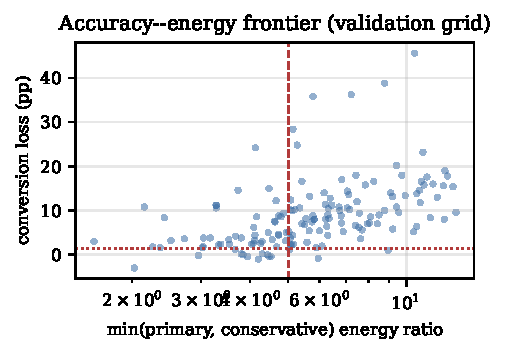
\includegraphics[width=\linewidth]{../figures/pareto.pdf}
\caption{Accuracy--energy frontier over the validation working-point grid. Dashed and dotted lines mark $5\times$ energy and $1.5$\,pp loss; points in the lower-right quadrant are the admissible high-energy-advantage region.}
\label{fig:pareto}
\end{figure}
\begin{figure}[b]
\centering
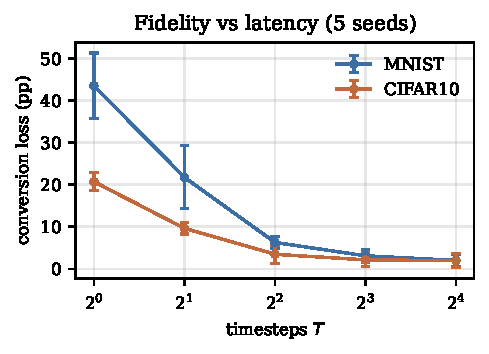
\includegraphics[width=\linewidth]{../figures/loss_T.pdf}
\caption{Conversion loss versus timesteps with five-seed error bars. Low $T$ is required for the energy advantage but increases loss.}
\label{fig:lossT}
\end{figure}
\section{Discussion}
\label{sec:discussion}

\textbf{Contribution of the combination.} Our starting components are not new individually. What is new is their joint behaviour on a graph-level visual operator. A linear pooling matrix leaves the error identity exact, so a formulation derived for node classification transfers without approximation; but a component that is beneficial in isolation can become harmful in the combination. The closed-form bias $\beta^\star$ cancels floor-quantisation error for an integrate-and-fire rate, whereas the deterministic two-phase schedule already delivers the exact count. Keeping both double-corrects the current. Identifying and removing this redundancy is a mechanistic contribution, not a hyperparameter choice: it is predicted by~\eqref{eq:dtp}, verified by a paired ablation, and consistent across both datasets and all seeds.

\textbf{Stability of the energy result.} The 45\,nm per-operation ratio is only \MACACRatio, so a $5\times$ advantage requires the SNN's total ACs to fall below the ANN's MACs. Two mechanisms achieve this together: a narrow trained network reduces the number of emitting units, and $T\in\{2,3,4\}$ bounds the number of propagation steps. Neither alone suffices. Reporting a conservative convention that also charges real-valued propagation as MACs is important, because an AC-only count can be made arbitrarily favourable by driving the network toward zero spikes. We exclude zero-spike and chance-level-teacher configurations.

\textbf{The accuracy--energy trade-off.} The frontier in Fig.~\ref{fig:pareto} makes the trade-off explicit: widening the network or lengthening the timestep improves fidelity but forfeits the energy advantage, while narrowing it has the opposite effect. Increasing the training budget, which we expected to stabilise the teacher, instead widened margins that the low-$T$ quantiser amplifies and worsened fidelity. This negative result delimits the regime in which the energy advantage is available.

\textbf{Limitations and threats to validity.} All energy figures are theoretical op-count estimates under a 45\,nm table; they ignore membrane-update cost, memory traffic and event-routing overhead, and are not measurements on neuromorphic hardware. Spike counts are therefore proxies. The method assumes a fixed non-negative linear adjacency and linear pooling; dynamic $k$-NN graphs, per-sample attention and max-relative aggregation break the factorisation in~\eqref{eq:identity} and are failure boundaries. Learning per-edge attention would require freezing it into a fixed operator first. Our teachers are deliberately small, so absolute accuracies are below published superpixel-GNN results. Finally, the four holdout groups are disjoint seeds drawn from the same two public benchmarks, so the conclusion is bounded to SuperPixel MNIST/CIFAR10 and does not establish ImageNet-scale behaviour. CUDA sparse reduction is non-deterministic; we mitigate it with five seeds, standard deviations and confidence intervals, and never select on a test split.

\section{Conclusion}
\label{sec:conclusion}

We studied whether a conversion framework assembled for graph node classification transfers to graph-structured visual classification, where images ship as superpixel graphs rather than regular grids, and whether it can deliver an ANN-relative energy advantage. A linear global pooling operator preserves the exact conversion-error identity $\Bh-B=\RAEW$; a unified float64 forward pass verifies it to \IdentityMax. Within the transferred combination we found a genuine mechanistic redundancy: deterministic two-phase spiking already realises the target firing count, so the closed-form bias $\beta^\star=\theta/(2T)$ double-corrects the rate and must be removed. With that correction, membrane decoding, margin regularisation and a narrow low-timestep network, both 45\,nm arithmetic-energy conventions exceed $5\times$ across four mutually disjoint holdout groups and \TotalSeeds\ independent seeds, while all adapted single-point conversion baselines remain near chance. The accompanying cost is an explicit accuracy--energy frontier, including a negative scaling result that delimits the low-timestep regime. The broader lesson is that conversion discretises a computation along the neighbourhood as well as along time: a component that is correct for one operator can be wrong for another. Extending the analysis to dynamic vision graphs and replacing op-count estimates with hardware measurements follow directly from this boundary.

{\small
\bibliographystyle{ieeenat_fullname}
\bibliography{references}
}
\end{document}
